%% ================================================================================================
%%  3. What no procedure can achieve
%%  Notes: research-agenda.md §3; proofs in A_proofs.tex
%%  Code: simulations/python/experiments.py (tables cw_probability, deadlock_n; figure fig_deadlock)
%% ================================================================================================
\section{What no procedure can achieve}\label{sec:limits}

Four families of results bound what a procedure can do. They explain why the literature offers
trade-offs rather than an optimum, and they fix the margins on which the choice of a procedure is made.

\subsection{Manipulation is always possible}

Arrow's theorem \citep{Arrow1951} rules out a rule that aggregates rankings into a ranking while
respecting unanimity, independence of irrelevant alternatives and non-dictatorship. Its strategic
counterpart is more directly relevant here: with three options or more, every rule that is onto and
not dictatorial can be manipulated, in the sense that some voter, in some profile, obtains a better
outcome by misreporting \citep{Gibbard1973,Satterthwaite1975}. The question is therefore not
\emph{whether} a procedure can be manipulated, but how often, by whom, and at what cost in
information and coordination. Computational hardness of manipulation has been proposed as a barrier
\citep{BartholdiToveyTrick1989manip}, but it is a worst-case notion that typical profiles do not
inherit \citep{FaliszewskiProcaccia2010}. Comparisons of rules therefore rest on the frequency of
manipulable profiles in realistic settings \citep{GreenArmytageTidemanCosman2016}, which is how
Section~\ref{sec:simulation} proceeds.

The majority principle has a specific cost: every Condorcet-consistent rule violates
\emph{participation} when there are four options or more, so that a group of voters can sometimes obtain
a better outcome by abstaining \citep[the no-show paradox,][]{Moulin1988noshow}; the bound is tight at 12
voters \citep{BrandtGeistPeters2017}. Rules that score options independently (plurality, Borda,
approval) satisfy participation but are not Condorcet-consistent.

\subsection{Majorities can cycle, but rarely do in structured electorates}

Between two options, simple majority is the only rule that is anonymous, neutral and positively
responsive \citep{May1952}. With three options or more, majority preferences can be cyclic: $A$ beats $B$,
$B$ beats $C$ and $C$ beats $A$ \citep{Condorcet1785}. Under the impartial culture, where every voter's ranking is drawn uniformly
and independently, a Condorcet winner exists in the limit of a large electorate with probability
91.2\% for three options and 74.9\% for five \citep{Guilbaud1952,GehrleinFishburn1976,Gehrlein2006},
and this probability falls towards zero as options are added. The impartial culture is a worst case:
preferences that share a structure produce Condorcet winners far more often. With single-peaked
preferences a Condorcet winner always exists, the option preferred by the median voter
\citep{Black1948}; in our two-dimensional spatial electorates it exists in more than 96\% of elections, even
with twelve options (Table~\ref{tab:cw_probability}). The empirical literature on real ballots reaches the same
conclusion: majority cycles are rare in practice \citep{RegenwetterEtAl2006,Tideman2006}, and spatial
models fit observed ballots better than the impartial culture \citep{TidemanPlassmann2012}. A procedure
must still say what to do in a cycle, but it is the exception it must handle, not the rule.

% Generated by simulations/python/experiments.py -- do not edit by hand
\begin{table}[htbp]\centering\small
\caption{Probability that a Condorcet winner exists}\label{tab:cw_probability}
\sbox{\tabbox}{\begin{tabular}{lrrrrrr}
\toprule
Culture & m = 3 & m = 4 & m = 5 & m = 6 & m = 8 & m = 12 \\
\midrule
Spatial (2D) & 99.8 & 99.7 & 99.4 & 99.0 & 98.5 & 97.4 \\
Polarised (55/45) & 99.7 & 99.5 & 98.9 & 98.1 & 97.6 & 96.0 \\
Impartial culture & 91.2 & 82.3 & 75.0 & 67.5 & 58.6 & 45.4 \\
Spatial (1D) & 100.0 & 100.0 & 100.0 & 100.0 & 100.0 & 100.0 \\
Impartial, $n\to\infty$ & 91.2 & 82.5 & 74.9 & 68.5 &  &  \\
\bottomrule
\end{tabular}}
\usebox{\tabbox}
\tabnotes{4,000 elections per cell, 101 voters; $m$ options including the status quo. Last row: the limit for an infinite electorate under the impartial culture \citep{GehrleinFishburn1976,Gehrlein2006}. Monte Carlo standard errors at most 0.8 points.}
{Monte Carlo simulation, cultures of \texttt{cultures.py}, rules of \texttt{voting.py}; last row from the literature; \texttt{experiments.py}.}
\end{table}


\subsection{Majority and minority veto are incompatible}

The first conflict between R1 and the majority principle is elementary.

\begin{proposition}[Majority versus minority veto]\label{prop:majority-veto}
Let $m \ge 3$ and $0 < \theta < 1/2$. There are profiles in which an option $x$ is the Condorcet winner,
$x$ is ranked last and vetoed by more than $\theta n$ voters, and another option is acceptable to every
voter. In such a profile no rule can both elect the Condorcet winner and avoid an option vetoed by at
least $\theta n$ voters when some option is vetoed by fewer. If, moreover, the minority's share exceeds
$1/m$, the Condorcet winner is outside the proportional veto core.
\end{proposition}

The proof (Appendix~\ref{app:proofs}) uses the profile of Example~E1 in Section~\ref{sec:examples}: 51
voters rank $A \pref B \pref C$, 49 rank $B \pref C \pref A$. $A$ beats every option, but 49\% of the
voters rank it last, while $B$ is everyone's first or second choice. A procedure must decide which of
$A$, the majority's option, and $B$, the compromise, is ``best''; any procedure that gives a minority of
size $\theta$ a veto elects $B$. \citet{KondratevNesterov2020} measure the same trade-off for common
rules: the share of voters that guarantees a majority its preferred options (majority power) against
the share that lets a minority exclude its least preferred options (veto power). In general, rules with
more majority power also have more veto power; proportional veto, Borda's rule and Black's rule are the
exceptions that trade majority power for minority protection.

\subsection{Stability and deadlock are two faces of the veto}

Veto rights make outcomes stable, and that is the problem. In a simple game, the core, the set of
options that no winning coalition wants to replace, is non-empty for every profile of preferences if
and only if the number of options is smaller than the game's \emph{Nakamura number}, the smallest number
of winning coalitions with an empty intersection \citep{Nakamura1979}. Majority rule has Nakamura number
3 (for $n \neq 4$), hence cycles; a quota rule that requires $q$ of the $n$ votes has Nakamura number
$\lceil n/(n-q) \rceil$; a game with a veto player has an infinite Nakamura number, hence a
non-empty core for any agenda. In spatial settings the same logic gives the supermajority thresholds that
guarantee an undominated option: a share above $d/(d+1)$ in $d$ dimensions for every profile
\citep{Greenberg1979}, and 64\% when the density of ideal points is concave \citep{CaplinNalebuff1988}.
Below these thresholds, simple majority in two or more dimensions has global cycles, and whoever controls
the agenda can lead the vote almost anywhere \citep{McKelvey1976,Plott1967}.

The stable outcome that a veto guarantees is, however, the status quo. With Euclidean preferences the
status quo cannot be unanimously improved upon as soon as it lies in the convex hull of the voters' ideal
points, and that event becomes certain as the assembly grows.

\begin{proposition}[Deadlock under unanimity]\label{prop:gridlock}
Let each voter $i$ have an ideal point $p_i \in \mathbb{R}^d$ and prefer options closer to it.
(i) If the status quo $\sq$ lies in the convex hull of $p_1, \dots, p_n$, no option is strictly preferred
to $\sq$ by every voter, so that unanimity with the status quo as default keeps $\sq$ whatever the
proposals. (ii) If the ideal points are drawn independently from a distribution whose support contains
a neighbourhood of $\sq$, the probability of (i) tends to one as $n \to \infty$.
\end{proposition}

Table~\ref{tab:deadlock_n} and Figure~\ref{fig:deadlock} quantify the speed: in our two-dimensional
electorates with seven proposals, unanimity keeps the status quo in 43\% of elections with three voters,
86\% with eleven and 99.6\% with 101. \citet{BuchananTullock1962} framed the choice of a voting quota as
a cost minimisation: the expected cost imposed on a member by decisions they oppose falls as the quota
rises towards unanimity, while the cost of reaching a decision rises with it. Proposition~\ref{prop:gridlock}
says the second cost becomes infinite in a large assembly: under individual veto the decision is never
reached. \citet{Rae1969} showed that simple majority is the rule that maximises a voter's expected
agreement with outcomes when the voter does not know their future position, the opposite corner of the
trade-off.

\begin{figure}[htbp]\centering
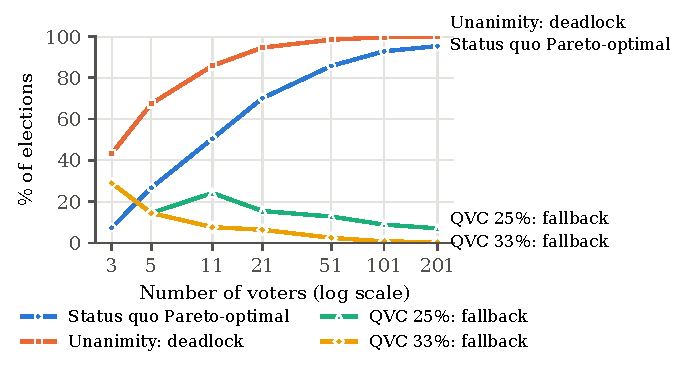
\includegraphics[width=0.85\linewidth]{fig_deadlock}
\caption{Deadlock under unanimity as the assembly grows}\label{fig:deadlock}
\figurenotes{Share of elections in which: the status quo lies in the convex hull of the voters' ideal
points, so that no option can be unanimously preferred to it (Proposition~\ref{prop:gridlock}); unanimity
with the status quo as default keeps it because no proposal is preferred to it by every voter; \QVC\ with
a blocking quota of 25\% or 33\% finds every option vetoed by the quota and falls back on the
least-vetoed options, still deciding. Spatial culture, 7 proposals and the status quo, 1,000 elections
per point. Values in Table~\ref{tab:deadlock_n}.}{Monte Carlo simulation, \texttt{experiments.py};
\texttt{figures.py}.}
\end{figure}
